\documentclass[12pt]{article}

\usepackage{graphicx}
\usepackage{float}
\usepackage{amsmath}
\usepackage{amssymb}
\usepackage{graphicx}
\usepackage[utf8]{inputenc}
\usepackage[spanish]{babel}
\usepackage{geometry}
\geometry{left=2cm,right=2cm,top=2cm,bottom=2cm}
\usepackage{listings}
\lstset{basicstyle=\ttfamily,
  showstringspaces=false,
  commentstyle=\color{red},
  keywordstyle=\color{blue}
}


\title{%
  Archivos OBJ\\
  \large Tarea 05 \\
    \Large Computación Gráfica\\
     \large UNAM 2022-2}
\author{Gibran Zazueta Cruz \\
\small 24/marzo/2022}
\date{}

\begin{document}
\maketitle

\section{Introducción}

El programa que se presenta a continuación recibe una malla 3d desde un archivo OBJ y lo renderiza dentro de una escena. Los objetos se definen en 3 archivos diferentes con geometría para un cubo de 8 vértices y 6 caras cuadradas, un cubo de 8 vértices y 12 caras triangulares y una esfera con caras rectangulares.

\begin{figure}[H]
\centering
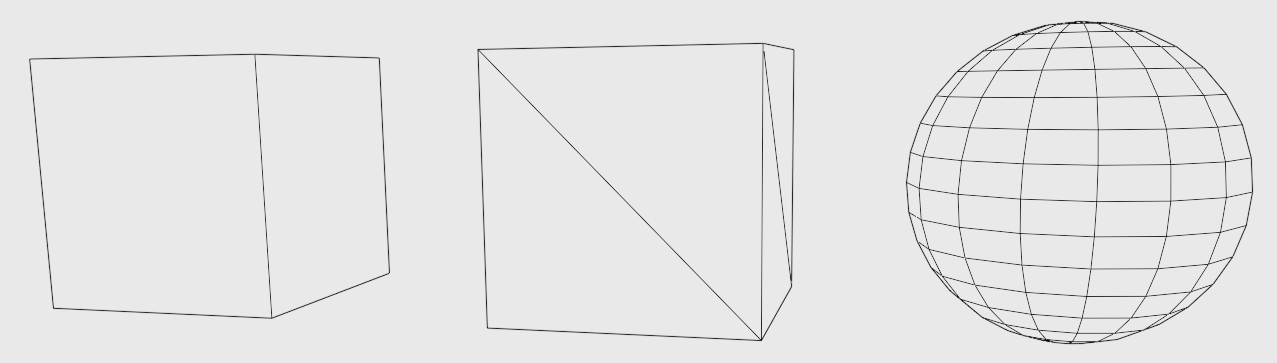
\includegraphics[scale=0.3]{images/objetos.png}
\caption{Objetos a renderizar}
\end{figure}


Como ya se mencionó, la geometría se lee desde un fichero OBJ. Se explica a continuación.

\subsection{Archivo OBJ}

OBJ es un formato de archivos desarrollado por Wavefront Technologies. Representa la geometría 3d definiendo:

\begin{itemize}
\item Posición de los vértivces
\item Normal de los vértices
\item Coordenadas UV de textura
\item Caras (como una lista de vértices)
\end{itemize}


Para este trabajo solo se hace uso de la posición de los vertices y la definición de las caras.


\subsubsection{Librería \textit{assimp}}

Para leer los archivos se utiliza la libreria de \text{assimp}. 
\textit{Assimp} es una librería open source que soporta multiples formatos de geometria 3d, entre llos .OBJ. Además funciona con diversos sistemas operativos y provee una interfaz de C++.

También soporta una jerarquía de nodos para mallas, materiales, texturas y animaciones de \textit{bones}. Para el programa de este reporte se hace uso principalmente de la función \textit{import} clase Assimp::Importer que almacena datos es una estructura llamada aiScene.


\section{Escena y materiales}

Los objetos cuentan con 2 posibles materiales a seleccionar, estos se definen dentro del código como:

\textbf{Material 1}
\begin{itemize}
\item Ambiental = {0.0, 0.0, 0.0, 1.0},
\item Difusa = {0.50, 0.50, 0.50, 1.0},
\item Especular {0.70, 0.70, 0.70, 1.0} 
\item $\rho$ = 32.0.
\end{itemize}


\textbf{Material 2}
\begin{itemize}
\item Ambiental = {0.23125, 0.23125, 0.23125, 1.0},
\item Difusa = {0.2775, 0.2775, 0.2775, 1.0},
\item Especular {0.773911, 0.773911, 0.773911, 1.0}
\item $\rho$ = 89.6.
\end{itemize}


Finalmente, la escena a renderizar cuenta con 2 luces (blanca y azul) y 3 cámaras.

Se disponen de la siguiente manera: 


\begin{figure}[H]
\centering
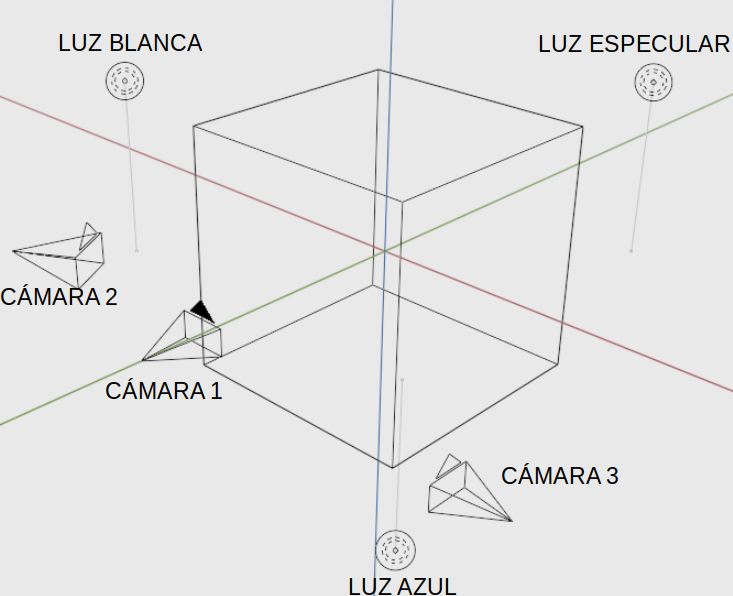
\includegraphics[scale=0.3]{images/ESCENAA.png}
\caption{Posición de las componentes de la escena}
\end{figure}



\section{Estructura del código}

Desde \textit{mainwindow.cpp} se llama a la función \textit{importFile()} que está definida en \textit{functions.cpp}. La función recibe el path del archivo (como una cadena std::string) y apuntadores al contenedor de vertices y caras del objeto cubeObject, que es el objeto  a renderizar en la escena. Dentro de esta función se utiliza la librería de assimp. Se importa la información del fichero con la función \textit{importer} de la clase Assimp::Importer  y se guarda la escena en una variable aiScene. La función \textit{importer} necesita que se le especifique un \textit{"Process"}, que es un post-procesado de los datos leidos. En este caso se utiliza \textit{aiProcessJoinIdenticalVertices} para unir los vértices iguales (que son los vértices que se repiten entre las caras). 
\\

La información del archivo se importa a la estructura de datos \textit{aiScene}. Dentro del programa la información de la geometría se procesa desde un objeto de la clase CubeObject. Esta clase tiene un método para calcular normales de las caras y normales de los vertices, por lo que solo es necesario darle información de lasOBJ coordenadas de los vértices y la composición de las caras.
\\

Después de esto, en mainwindow se crean los objetos de clase \textit{light} para las luces blanca, azul y especular, se especifican intensidad, color y posicionamiento. También se crea el grid de botones que conforma la GUI de la aplicacion. Finalmente se llama a la funcion \textit{drawObject()} con un timer que renderizará al polígono cada 30 ms.
\\

En la funcion  \textit{drawObject()} se llama a la función pipeline del objeto raster. En la funcion pipeline primero se proyectan los vertices dentro del objeto de cámara (que contendrá el marco de referencia correspondiente a la cámara 1, 2 o 3),
despues se hace el scan conversion e interpolación de los pixeles, zbuffer, normales e información de color(si es que se usa Gouroud).

Si no se utiliza gouroud el último paso es calcular el sombreado de phong en cada pixel.
\\

Finalmente, la informacion de posición de pixeles, color y profundidad se pasa a la clase renderwindow(que hereda de QPainter), donde se pintarán los pixeles sobre el canvas.




\section{Ejecutar el programa}
En la carpeta de build se puede ejecutar el programa con el archivo renderOBJ-Run. Desde la consola de comandos de linux:

\begin{lstlisting}[language=bash,title={bash}]
./renderOBJ-Run
\end{lstlisting}


En la carpeta principal está el código fuente. Para generar el ejecutable primero se genera el Makefile con

\begin{lstlisting}[language=bash,title={bash}]
 qmake renderOBJ.pro
\end{lstlisting}

Después se construye el proyecto con \textit{make}



\section{Instrucciones de uso}
Se presenta la interfaz del programa.

\begin{figure}[H]
\centering
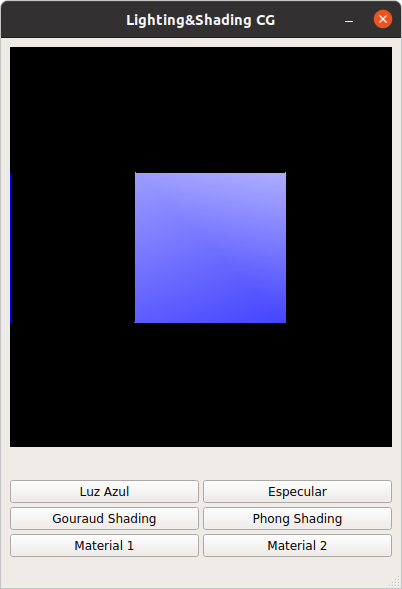
\includegraphics[scale=0.5]{images/gui.png}
\caption{Interfaz gráfica del programa}
\end{figure}

Para cambiar entre las camaras se utilizan las teclas de los numeros
\begin{itemize}
\item "1". Cambia a la cámara 1
\item "2". Cambia a la cámara 2
\item "3". Cambia a la cámara 3

\end{itemize}

 

Para rotar el objeto sobre el eje X se presiona la tecla R. Se vuelve a apresionar para que deje de rotar.
\\

Los botones \textit{Luz Azul} y \textit{Especular} encienden o apagan las luces correspondientes. El programa inicia con todas las luces activas.
\\

\textit{Gouraud Shading} activa el Sombreado por Gouraud y \textit{Phong Shading} el sombreado de Phong.
\\

Es posible cambiar entre archivos desde el código. En la variable path de mainwindow se cambia la extension por el archivo correspondiete. Por defecto es $Cube\_Triangle$, los otros dos son $Cube\_Quads$ y sphere.



\section{Programa en ejecución}

\begin{figure}[H]
\centering
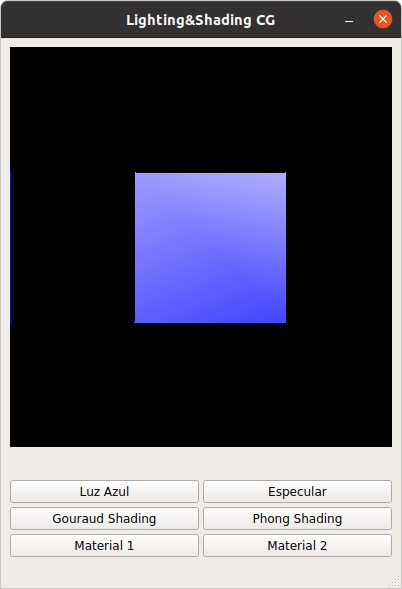
\includegraphics[scale=0.5]{images/ej1.png}
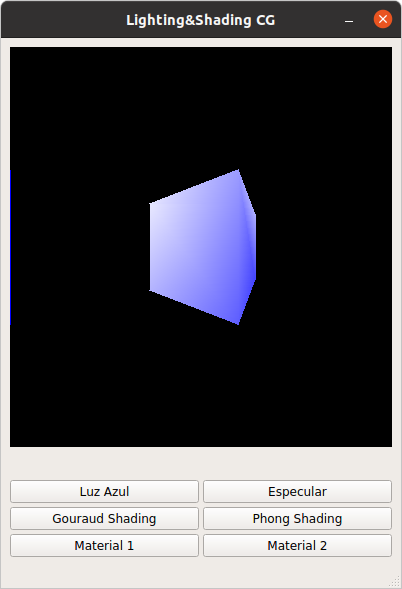
\includegraphics[scale=0.5]{images/ej2.png}
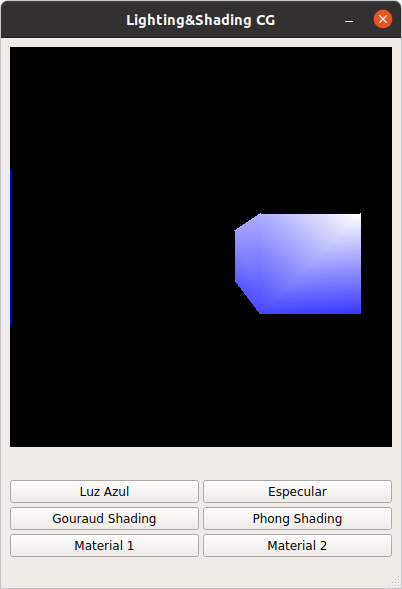
\includegraphics[scale=0.5]{images/ej3.png}
\caption{Gouraud Shading. Cámara 1, 2 y 3. Material 1}
\end{figure}


\begin{figure}[H]
\centering
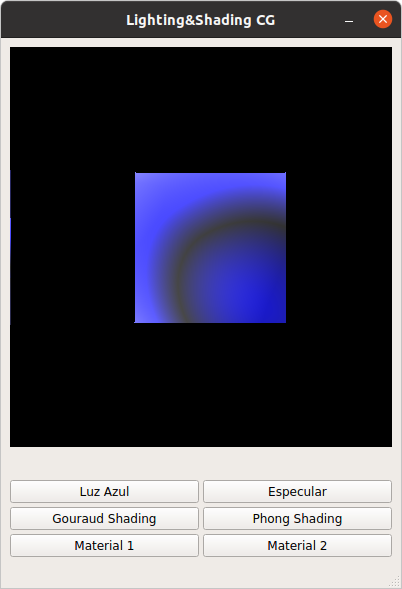
\includegraphics[scale=0.5]{images/ej4.png}
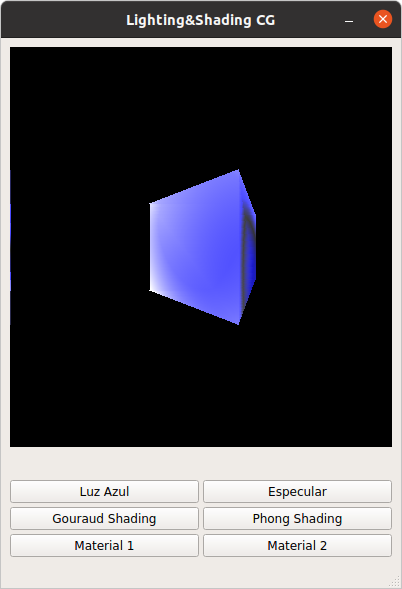
\includegraphics[scale=0.5]{images/ej5.png}
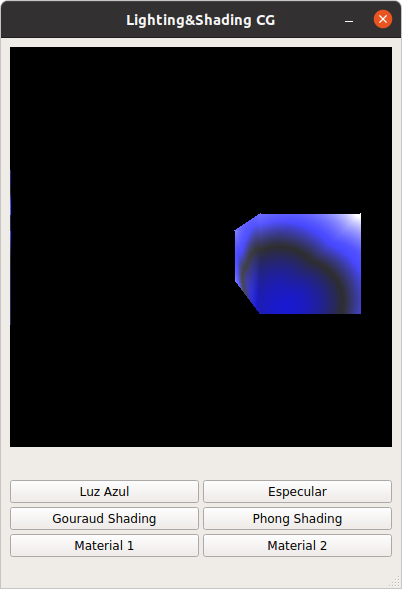
\includegraphics[scale=0.5]{images/ej6.png}
\caption{Phong Shading. Cámara 1, 2 y 3. Material 2}
\end{figure}


\begin{figure}[H]
\centering
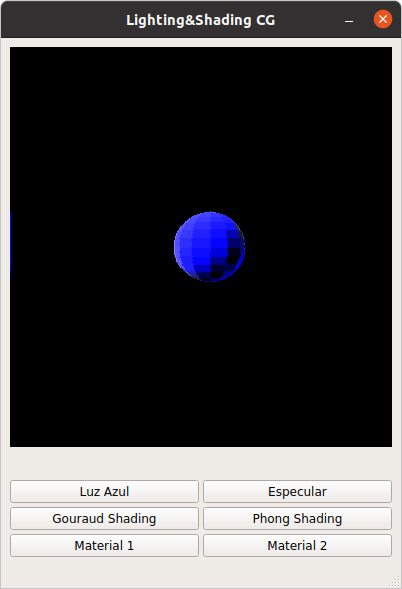
\includegraphics[scale=0.5]{images/esfera.png}

\caption{Renderizado esfera}
\end{figure}

\begin{thebibliography}{99}


%\bibitem{open} Wavefront obj file. ($https://en.wikipedia.org/wiki/Wavefront_.obj_file$)

\end{thebibliography}


\end{document}